\newpage

\section{Ferro e Leghe Metalliche}

\subsection{Proprietà fisiche}

L'acciaio è una lega ferro-carbonio che presenta molte fasi differenti in base alla temperatura e composizione. La percentuale massimo di carbonio è 6,67\%. Questa percentuale non è casuale ma rappresenta la percentuale per ottenere un composto intermetallico Fe-C, la cementite Fe$_3$C. Al di fuori di questa percentuale si ha la formazione di grafite.
\begin{figure}[h]
    \centering
    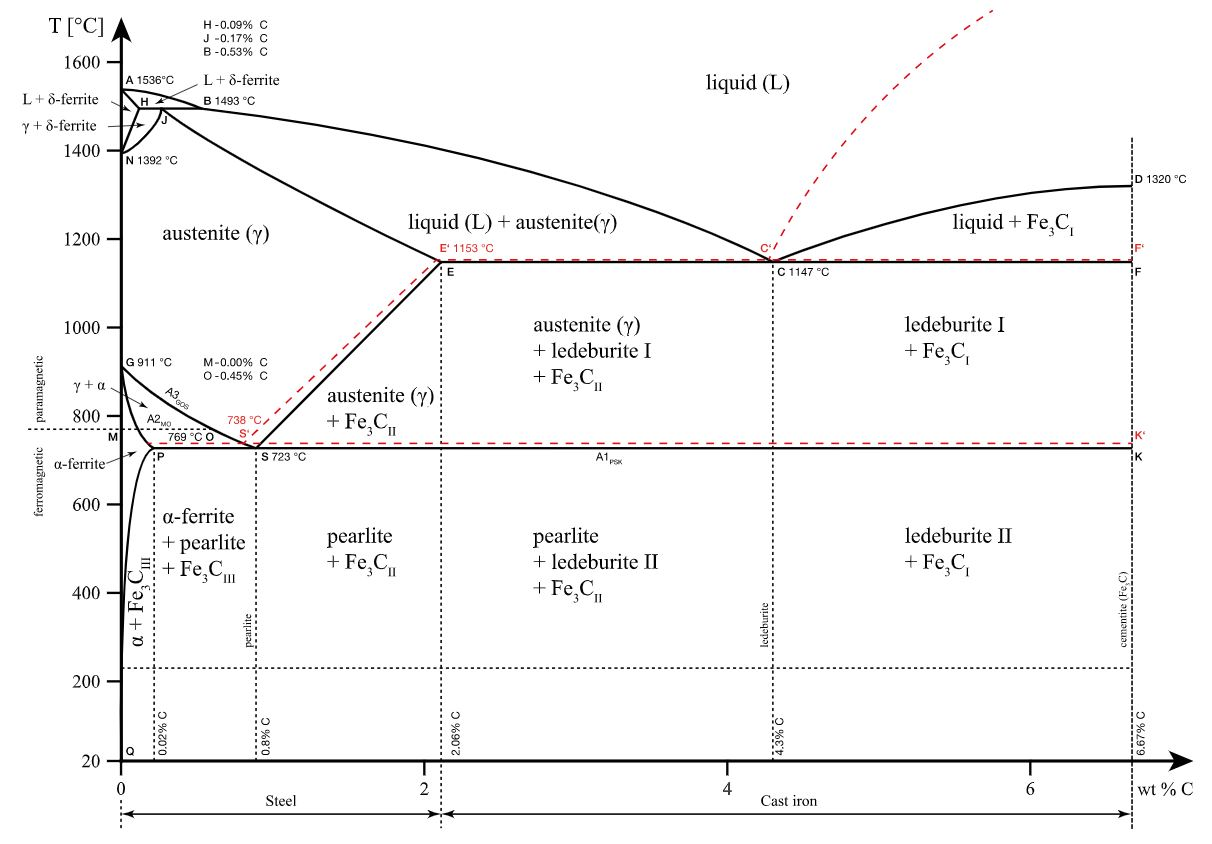
\includegraphics[width=10cm]{acciaio e transizioni di fase/Fe_phase_diagram.jpg}
    \caption{Diagramma di fase dell'acciaio.}
    \label{Steel-PhDia}
\end{figure}
Possiamo fare alcune semplici considerazioni da Fig \ref{Steel-PhDia}:
\begin{itemize}
    \item l'acciaio fonde a temperatura più elevata della ghisa (2.1\% determina il confine).
    \item l'acciaio è polimorfo e presenta più forme: Ferrite-$\delta$ (BCC), Ferrite-$\alpha$ (BCC), austenite $\gamma$ (FCC). Da notare che il passaggio da una forma cristallina all'altra comporta tensioni, in particolar modo quando la struttura cristallina è differente; inoltre è rilevante il fatto che la ferrite $\delta$ abbia un passo reticolare maggiore rispetto alla ferrite $\alpha$.
    \item La cementite $Fe_3C$ è un materiale termodinamicamente instabile ma cineticamente inerte e quindi non decompone.
    \item La solublità del carbonio nel ferro risulta incredibilmente bassa (0,02\% a 700°C), questa cosa non deve stupire in quanto il ferro è BCC e le posizioni interstiziali non sono favorevoli.      
\end{itemize}
Vediamo di capire cosa accade se raffreddiamo il nostro campione. Supponiamo di trovarci a 1000°C a concentrazione eutettoidica e raffreddiamo sotto 700 gradi, in questo caso si ottiene una struttura lamellare $\alpha$ + Fe$_3$C (perlite). La forma $\alpha$ risulta essere duttile mentre la cementite è dura e fragile ed è quest'ultima a impartire importanti proprietà di durezza agli acciai.
Se invece siamo in condizioni ipoeutettoidiche si avrà una nucleazione sui bordi di grano della componente maggioritaria (austenite), viceversa in condizioni ipereutettoidiche si avrà la nucleazione di cementite nei bordi di grano.

\subsection{Curve di Bain}

Le curve di Bain o curve TTT (time temperature transition) sono curve che descrivono le forme cristallina dell'acciaio che otteniamo a partire dalla composizione chimica e dal profilo di raffreddamento (veloce o lento).
vediamo di commentare un poco questo grafico (fig. \ref{Bain-Curves}):
\begin{itemize}
    \item La prima temperatura incontrata (720°C) è la temperatura al di sotto della quale l'austenite non è più stabile. Ogni struttura al di sotto della temperatura critica è comunque in forma $\alpha$ + Fe$_3$C.
    \item M$_s$ rappresenta la curva alla quale si ha l'inizio della transizione austenite $\rightarrow$ martensite, M$_f$ ne rappresenta la fine. Similmente sono le curve per la bainite e per la perlite. Bainite e perlite differenziano per la struttura, che è rispettivamente aciculare e lamellare.
    \item Esistono due forme differenti sia per la \textbf{\textit{perlite}} che per la \textbf{\textit{bainite}}. Se il raffreddamento è lento e diamo modo a far crescere i cristalli otteniamo la perlite grossolana, nell'altro caso otteniamo la perlite fine che presenta proprietà meccaniche superiori. La superiorità meccanica della perlite fine è dovuta alla maggior percentuale di superficie a contatto nei bordi di grano essendo la cementite e la ferrite fortemente legati tra loro. La bainite può esistere anch'essa in due forme: gli aghi possono essere paralleli al grano o ruotati di 45°. In generale le bainiti sono più lavorabili rispetto la martensite e presentano discrete proprietà a causa della cementite che rafforza la struttura.
\end{itemize}

\begin{figure}
    \centering
    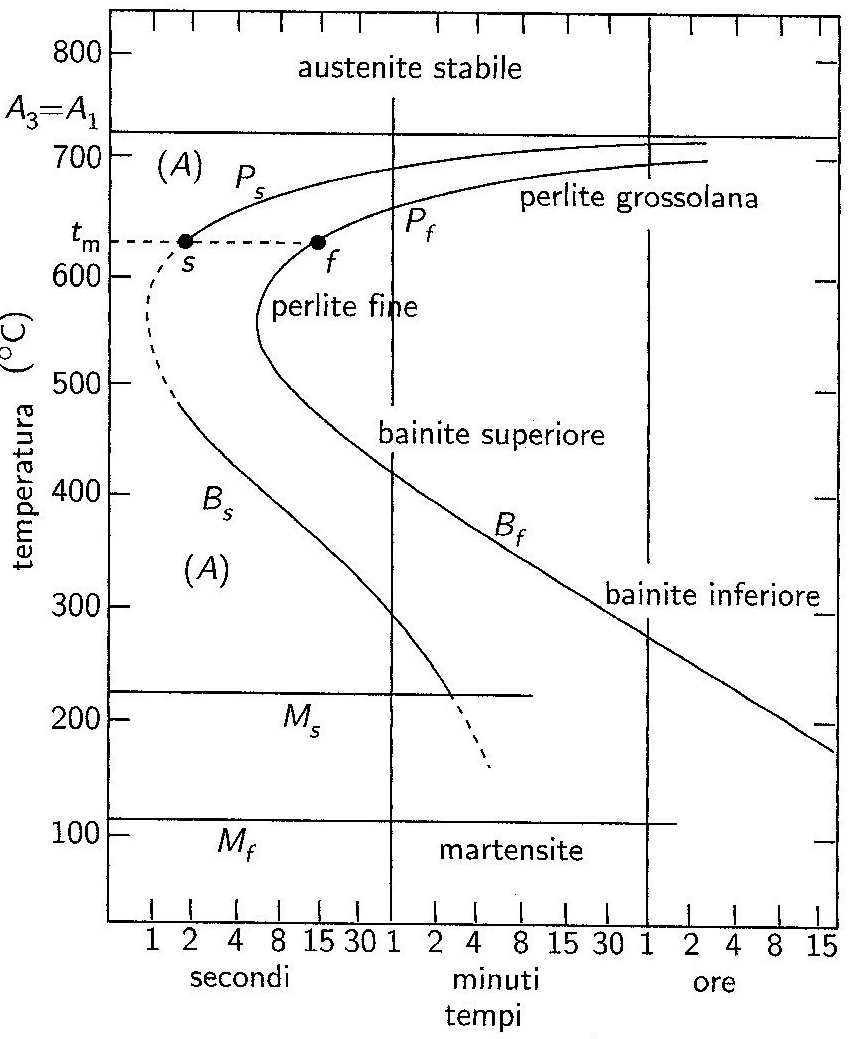
\includegraphics[height=10cm]{acciaio e transizioni di fase/Curve_bain.png}
    \caption{Curve di Bain}
    \label{Bain-Curves}
\end{figure}

La \textbf{\textit{martensite}} si ottiene per raffreddamento molto veloce, senza permettere la trasformazione da $\gamma$ a $\alpha$. Non si fornisce sufficiente tempo al metallo per riorganizzare la struttura cristallina da FCC a BCC, difatti si ottiene invece una forma intermedia (TCC, tetragonale a corpo centrato).
Questo risultato è stato ottenuto studiando i sistemi di scorrimento. 
La presenza di una maggiore quantità di carbonio aumenta l'intensità della deformazione e quindi ostacola maggiormente le dislocazioni, rendendo però il sistema più fragile.
Da notare che la possibilità di ottenere la martensite non è da ritenersi scontata, difatti se la temperatura martensitica finale (M$_f$) fosse al di sotto della temperatura ambiente non avremmo la possibilità di completare la nostra transizione ed a causa del differente volume di cella otterremo una frattura del sistema.
Per riuscire a risolvere questo problema si possono aggiungere elementi di lega, che vengono definiti:
\begin{itemize}
    \item $\gamma$-geni se aumentano l'area della zona $\gamma$ (il carbonio ad esempio, rimanendo però sotto il 2.1\%).
    \item $\alpha$-geni se aumentano l'area della ferrite.
\end{itemize}
Infatti le curve di Bain hanno una forze dipendenza dalla presenza di eventuali ulteriori specie all'interno della lega in quanto modificano il punto eutettoidico e e la temperatura eutettoidica.

\subsection{Martensite}

La martensite è ottenuta dal rapido raffreddamento della austenite (chiamata anche \textit{\textbf{tempra}}). La presenza del carbonio conferisce a questo materiale un grande punto di snervamento e grande resistenza (questi punti praticamente coincidono). Il sistema però risulta fragile e non riesce ad immagazzinare molta energia.
Esistono diversi modi di operare per aumentare il comportamento plastico dell'acciaio:
\begin{itemize}
    \item \textbf{\textit{Rinvenimento}}: Si procede al riscaldamento dell'acciaio a diverse centinaia ma comunque al di sotto della temperatura austenitica. Questo serve solamente a riattivare i moti diffusivi all'interno dell'acciaio in modo da ridurre la tensione all'interno del materiale e aumentarne la duttilità. La ripetizione di operazioni di rinvenimento e tempra è chiamata \textbf{\textit{bonifica}}.
    Da notare che il rinvenimento non elimina tutti gli effetti ottenuti dalla tempra in quanto rimaniamo sempre al di sotto della temperatura di transizione di fase. Gli acciai da bonifica vengono usati per fare gli alberi delle meccaniche e meccanismi di trasmissione a causa della loro proprietà di immagazzinare l'energia superiore a quello fresco. La forma martensitica fresca viene invece usata per fabbricare molle grazie alla loro elevata resistenza ed al loro comportamento quasi solo lineare.
    \item \textbf{\textit{Ricottura}}: in questo caso si riscalda ad una temperatura maggiore di quella austenitica e si procede ad un riscaldamento controllato. La ricottura elimina tutti gli effetti della tempra.
    \item \textbf{\textit{Distensione}}: in questo caso si procede a riscaldare il materiale ad una temperatura relativamente bassa (100-150 °C); il materiale è ancora fragile ma acquisisce una piccola porzione plastica.
\end{itemize}
Oltre a questi esistono anche altri metodi come il raffreddamento dell'austenite all'aria, detto normalizzazione (produce perliti molto fini).
\begin{figure}
    \centering
    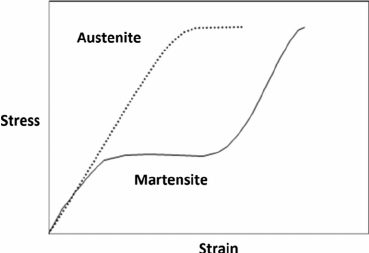
\includegraphics[width=8cm]{acciaio e transizioni di fase/Austenite-Martensite.png}
    \caption{Curva di elasticità di Austenite e Martensite}
    \label{fig:enter-label}
\end{figure}
Riattivare i processi diffusivi all'interno di un materiale ne migliora la lavorabilità e la duttilità ma ne peggiora le proprietà meccaniche. Ricordiamo però che la rigidezza non varia molto tra le varie forme dell'acciaio, dato che dipende principalmente dalle interazioni atomiche.

\subsection{Prova di temprabilità o prova Jominy}

Viene utilizzata per capire l'effetto della tempra sul materiale. Un provino fissato che si al di sopra della temperatura austenitica viene raffreddato spruzzando acqua a 24°C creando di fatto un gradiente di temperatura sulla superficie (il campione non sottoposto al raggio diretto viene raffreddato per conduzione). Successivamente viene misurata la durezza lungo l'asse.

\begin{figure}[h]
  \begin{minipage}[b]{0.5\linewidth}
    \centering
    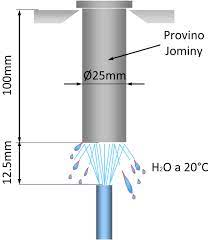
\includegraphics[width=0.6\linewidth]{acciaio e transizioni di fase/jominy test.jpg}
    \label{jominy-test}
  \end{minipage}
  \begin{minipage}[b]{0.5\linewidth}
    \centering
    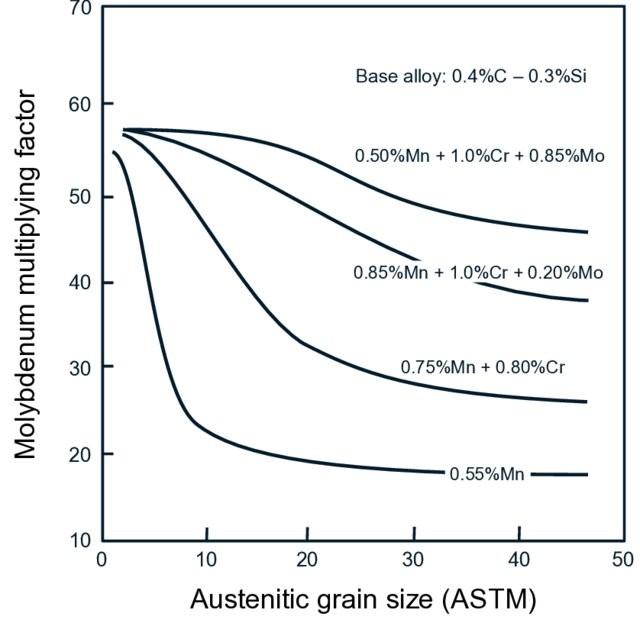
\includegraphics[width=0.7\linewidth]{acciaio e transizioni di fase/JOMINY-chart.jpg}
    \label{jominy-chart}  

  \end{minipage}
  \caption{Sinistra: setup del test. Destra: curve ottenute aggiungendo elementi di lega}
\end{figure}

All'aumentare della distanza aumenta la \% austenitica con una conseguente diminuzione della durezza. In questo test si cerca di limitare eventuali correnti convettive che trasformano le fasi austenitiche in perliti o bainiti a causa di un eccessivo raffreddamento.

\subsection{Classificazione degli acciai}

Gli acciai possono essere classificati secondo diverse categorie:
\begin{itemize}
    \item Composizione chimica (quando è nota): C\textit{X} dove \textit{X} è la $\%$ di carbonio moltiplicata per 100, o \textit{X}MgNi\textit{YZ} dove \textit{X,Y,Z} sono rispettivamente i valori percentuali moltiplicati per un fattore 100 per il carbonio e variabile per gli altri elementi di lega (si dice altamente legato se siamo sopra 5$\%$ in peso).
    \item Proprietà meccaniche (Fe250:$\sigma_R$=250 o FeE200:$\sigma_y$200). Elementi di lega come V o Cr aumentano la rigidezza del'acciaio.
    \item Gli acciai inox.
\end{itemize}

Ci sono poi gli acciai per molle: ovviamente essendo una molla vogliamo che lavori sempre in regime lineare: gli acciai martensitici freschi presentano questo tipo di comportamento; spesso si effettua una distensione per aggiungere un pezzettino plastico.
Per formare acciai duri si cerca di formare precipitati duri con opportune specie chimiche (come CW) oppure aggiungendo altro carbonio. Il trattamento viene eseguito con l'obiettivo di ottenere il picco di durezza alla temperatura di lavoro.

\subsection{Acciai inox}

Gli acciai inox sono acciai ottenuti usando il Cr come elemento di lega in proporzione maggiore del 12$\%$. Il cromo forma una patina passivante che protegge l'acciaio dalla corrosione impedendo la formazione della ruggine con conseguente rottura del materiale. Perché si formi questo strato omogeneo di cromo sulla superficie è necessario che la percentuale sia maggiore di 12 in ogni punto del materiale. La presenza di cromo comporta importanti cambiamenti al diagramma di fase dell'acciaio; bisogna comunque sempre tenere sotto controllo la quantità di cromo presente, in quanto il cromo tende a precipitare assieme al carbonio nei bordi di grano diminuendo la quantità presente nel manufatto e favorendone la degradazione.
Per evitare ciò è possibile agire:
\begin{itemize}
    \item riscaldando e sciogliendo i precipitati (non aggiusta eventuali danni ed è costoso).
    \item Usando poco carbonio (non permette però di ottenere la martensite)
    \item Utilizzando anche altri elementi di lega più affini di Cr al carbonio (ad esempio Ti).
\end{itemize}

\begin{figure}
    \centering
    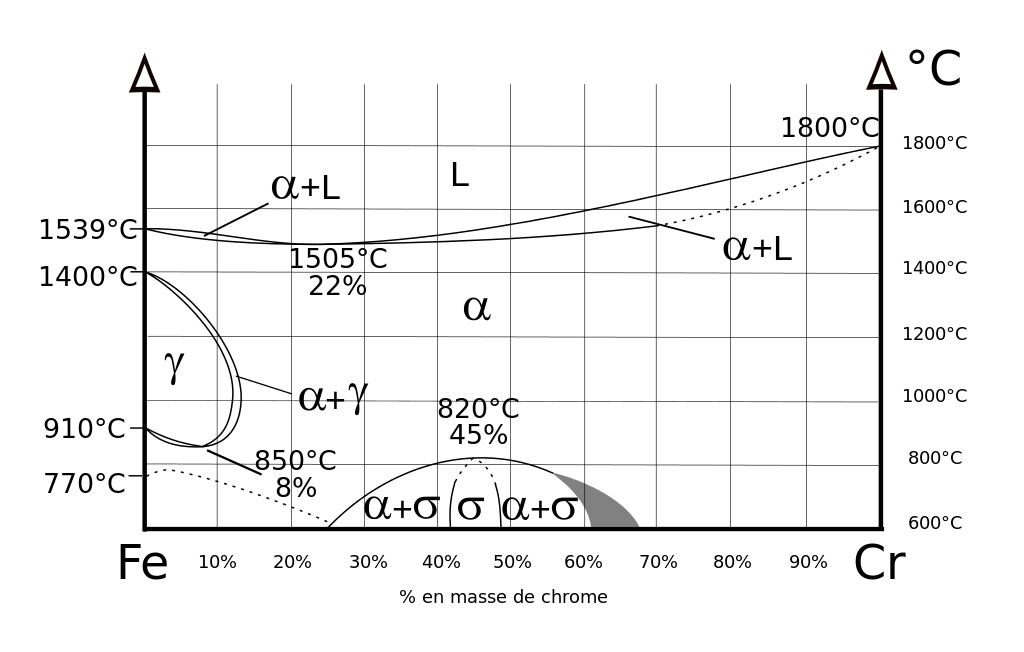
\includegraphics[width=10cm]{acciaio e transizioni di fase/Diagramme_phase_Fe.png}
    \caption{Diagramma di fase dell'acciaio inox.}
    \label{acciaio-inox.}
\end{figure}

Ci sono tre tipi di acciai inox:
\begin{itemize}
    \item Ferritici: 13\%$<$Cr$<$25\%. Sono molto dolci e poco usati a causa delle scarse proprietà meccaniche (comunque ha E=204GPa). Spesso è utilizzato come rivestimento per sistemi che non devono sopportare grandi carichi.
    \item Martensitici: non sempre sono ottenibili in quanto si ottengono per bassi tenori di cromo. Si agisce aumentando il quantitativo di carbonio che è $\gamma$-geno. Sono usati per produrre strumenti molto duri con buona resistenza alla corrosione come i bisturi o posate.
    \item Austenitici: Possono subire grandi deformazioni plastiche e contengono quantitativi di cromo importanti 18\%<Cr<25\% oltre a nichel 10\%<Ni<20\%
    \end{itemize}
Le curve di Bain in questo caso sono molto distanti e i tempi di transizione per la bainite e perlite si spostano a scale temporali molto lunghe rendendo di fatto l'austenite stabile indipendentemente dalla velocità di raffreddamento (non si vede quindi una transizione duttile-fragile). 

\subsection{Invecchiamento leghe leggere}

In leghe di Al (maggioritario) e Cu (minoritario) è possibile far precipitare il soluto (bassi contenuti, attorno al 4\%) aumentando la T.
In questo modo attraverso i moti diffusivi si genera un precipitato coerente $\theta$ che rende il materiale più resistente alle deformazioni. Aumentando troppo T si genera però un precipitato che non è più coerente $\theta"$ che rende il materiale più fragile.
In generale possiamo riassumere il processo:
\begin{itemize}
    \item Si hanno $\%$ di soluto contenute.
    \item Il processo è controllato.
    \item Si deve avere la possibilità di ottenere un precipitato coerente.
\end{itemize}

\subsection{Ghise}

Le ghise presentano una percentuale di acciaio maggiore dell'acciaio, risultando più dure ma anche più fragili (lavorano meglio con carichi statici).
Le ghise non sono saldabili e si lavorano male con macchine utensili, pertanto si lavorano per fusione. Le ghise usano per applicazioni industriali hanno un tenore che va da circa il 2.2\% al 4\%; al di sopra il tenore di carbonio è troppo elevato per utilizzi pratici.
\begin{itemize}
    \item \textbf{\textit{Ghisa grigia}}: presenta grafite in fiocchi e presenta una durezza molto elevata. Viene usata come come ammortizzatore
    \item \textbf{\textit{Ghisa globulare}} (o sferoidale): il carbonio non prende la forma di fiocchi ma di sfere. Viene principalmente usato come elemento strutturale a causa dell'elevata resistenza (350-450 MPa). 
    \item \textbf{\textit{Ghisa bianca}}: Il carbonio si trova sotto forma di cementite, sono molto fragili e si usa per ruote di carrelli o cilindri per la laminazione. Se portata a T di 800-900 °C per periodi lunghi si ha la sua solubilizzazione e si ottiene una struttura simile agli acciai da bonifica ottenendo un materiale molto più duttile.
\end{itemize}

\subsection{Lavorazione degli acciai}

L'acciaio è ottenuto a partire da vari minerali che vengono fusi nell'altoforno in cui il ferro si trova principalmente nella forma di ossido Fe$_2$O$_3$ e Fe$_3$O$_4$. Il combustibile è il carbon coke e il comburente è l'aria.  All'interno dell'altoforno la T aumenta man mano, alle temperature di lavoro si hanno le seguenti reazioni:

$$C+O_2\rightarrow CO_2$$
$$C+CO_2\rightarrow 2CO$$
$$3Fe_2O_3+CO\rightarrow 2Fe_3O_4+CO_2$$
$$Fe_3O_4+CO\rightarrow 3FeO+CO_2$$
$$FeO+CO\rightarrow Fe+CO_22$$

Ovviamente non sono le uniche reazioni che avvengono ma sono quelle che conducono alla formazione della ghisa. Oltre alla ghisa fusa si ottengono anche le scorie che galleggiano sopra la ghisa e vengono rimosse. La ghisa grezza (o grigia) appena uscita dall'altoforno trova scarsa applicazione industriale, poiché ha tenori di carbonio molto elevati e si trova sotto forma di fiocchi di grafite; tuttavia trova impiego come ammortizzatore di vibrazioni.